\documentclass[11pt]{article}
\usepackage{graphicx}
\usepackage{color, soul}
\usepackage{amsmath}
\usepackage{systeme}
\usepackage{spalign}
\usepackage{listings}
\usepackage{nicefrac}
\usepackage{empheq}
\usepackage[most]{tcolorbox}

\title{\vspace{-3.0cm}Report for Benjamin}
\author{Riccardo Di Dio}
\date{\today}

\begin{document}
\maketitle
\section{RC model}
The schematic of the model can be seen in figure\ref{fig:LungModelRC}
where $V_g(t)$ represents the difference in pressure between athmosphere and pleural pressure while $i_0(t)$ is the respiratory flow. $R_0$ is the resistance of the trachea, $R_1$ and $R_2$ the resistances of the bifurcations. The resistances can be  gotten by Poiseuille: $R_i = \frac{8\eta L_i}{\pi r_i^4}$. $C_1$ and $C_2$ are the compliances of the 2 compartments.
\begin{figure}[ht]
\label{fig:LungModelRC}
\centering
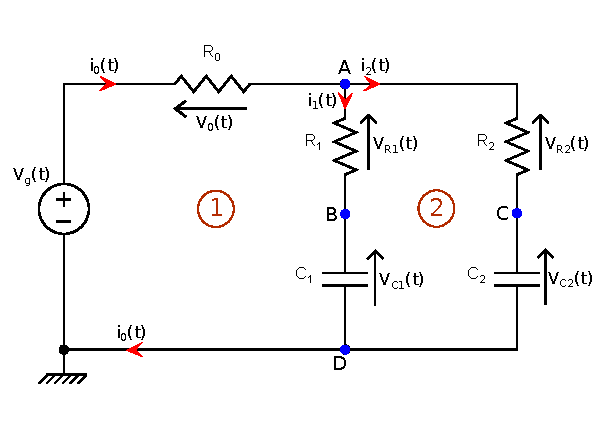
\includegraphics[scale=1.3]{LungModelRC.pdf}
\caption{Electrical equivalent of a bifurcation. 2 compartments are studied.}
\end{figure}
\section{Solving ODE in current}
\begin{figure}[!th]
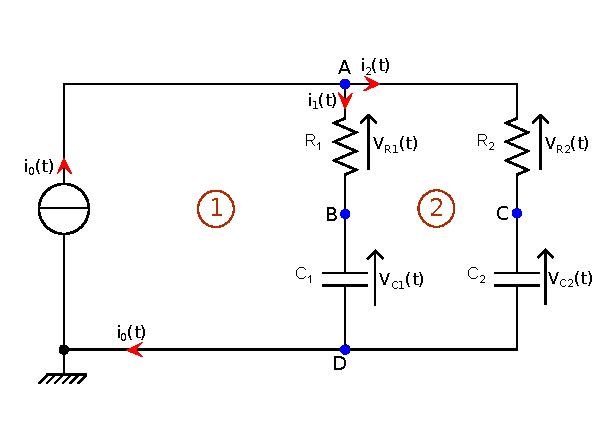
\includegraphics[scale=1.3]{TheveninEquivalent.pdf}
\caption{Thevenin equivalent of the circuit in figure 1. The voltage generator and $R_0$ are replaced in favor of a generator of current which simulate the airflow in the trachea.}
\end{figure}
LKI and LKV equations:
\begin{equation}
\label{eq:LKIandLKV}
  \spalignsys{
  	i_0 = i_1 + i_2;
  	V_{R_1} + V_{C_1} - V_{R_2} + V_{C_2} = 0
  }
\end{equation}
Components:
\begin{equation}
\label{eq:components}
  \spalignsys{
	i_1 = V_{R_1}/R_1 = dQ_1/dt;
	i_2 = V_{R_2}/R_2 = dQ_2/dt
  }
\end{equation}
Combining the equations:
\begin{equation}
\label{eq:big}
R_1i_1 + \frac{1}{C_1}\int_{t_0}^{t_1}i_1(\tau)\mathrm{d\tau} - R_2i_2 - \frac{1}{C_2}\int_{t_0}^{t_1}i_2(\tau)\mathrm{d\tau} = 0
\end{equation}
By deriving equation \eqref{eq:big} over time:
\[
\frac{di_1}{dt}R1 + \frac{i_1}{C_1} - \frac{di_2}{dt}R_2 - \frac{i_2}{C_2} = 0
\]
Remembering the LKI and using the conservation of charge: 
$$Q_0 = Q_1 + Q_2 \Rightarrow \frac{di_0}{dt} = \frac{di_1}{dt} + \frac{di_2}{dt}$$
\[
\spalignsys{
\frac{di_1}{dt}R_1 + \frac{i_1}{C_1} - \frac{di_2}{dt}R_2 - \frac{i_2}{C_2} = 0;
\frac{di_2}{dt}R_2 + \frac{i_2}{C_2} - \frac{di_1}{dt}R_1 - \frac{i_1}{C_1} = 0
}
\]
\vspace{1em}
\[
\spalignsys{
\frac{di_1}{dt}(R_1+R_2) + i_1(\frac{1}{C_1} + \frac{1}{C_2}) = R_2\frac{di_0}{dt} + \frac{i_0}{C_2};
\frac{di_2}{dt}(R_1+R_2) + i_2(\frac{1}{C_1} + \frac{1}{C_2}) = R_1\frac{di_0}{dt} + \frac{i_0}{C_1}
}
\]
\vspace{1em}
\[
\spalignsys{
\frac{di_1}{dt} + i_1\frac{\frac{1}{C_1} + \frac{1}{C_2}}{R_1 + R_2} = \frac{R_2\frac{di_0}{dt} + \frac{i_0}{C_2}}{R_1 + R_2};
\frac{di_2}{dt} + i_2\frac{\frac{1}{C_1} + \frac{1}{C_2}}{R_1 + R_2} = \frac{R_1\frac{di_0}{dt} + \frac{i_0}{C_1}}{R_1 + R_2}
}
\]
\begin{empheq}[box=\tcbhighmath]{equation}
\spalignsys{
\frac{di_1}{dt} = \frac{R_2\frac{di_0}{dt} + \frac{i_0}{C_2} - i_1(\frac{1}{C_1} + \frac{1}{C_2})}{R_1 + R_2};
\frac{di_2}{dt} = \frac{R_1\frac{di_0}{dt} + \frac{i_0}{C_1} - i_2(\frac{1}{C_2} + \frac{1}{C_1})}{R_1 + R_2};
}
\end{empheq}
Here we get a system of differential equations in which $R_1, R_2, C_1, C_2$ and $i_0$ are known and we can get the flow in the 2 different compartments.
\section*{Testing the differential equations in Python}
\end{document}